\section{Related work}

\textbf{Grounding Instructions to Robot Control.} Traditional approaches for grounding instructions assume a symbolic description of the environment state 
and robot actions. 
%
These approaches learn to associate phrases in an instruction with symbols conveying their meaning from 
annotated datasets. 
%
For example, \cite{howard2014natural,paul2016efficient,tellex2011approaching} map language to discrete motion constraints that can be provided to a motion planner for trajectory generation, \cite{matuszek2013learning,knepper2013ikeabot} parse language to a logical parse that includes  robot control actions and \cite{gopalan2018sequence,williams2018learning} use sequence to sequence modeling to ground language to LTL formulae capturing high-level task specifications. 
%
In contrast to such approaches, our work doesn't assume a symbolic model of the world and learns spatial and visual concepts and action semantics from data. 

\textbf{Inferring Plans from Instructions.} Another set of approaches focus on multi-stage tasks (e.g., cooking, assembly etc.) and propose 
learners that can infer action sequences by observing human task demonstrations. 
%
The work in ~\cite{paxton2019prospection} proposes a recurrent neural architecture that converts a natural language instruction to a sequence of intermediate goals for robot execution. 
%
Efforts such as \cite{shah2018bayesian,wang2020learning,kress2008translating} learn LTL task specifications from humans demonstrations and introduce a model for effectively searching in the space of programs. 
%
In another effort, ~\cite{lazaro2019beyond}, authors introduce a cognitively-inspired approach that infers 
a likely program from a symbolic generative grammar for a robot manipulator to form and re-arrange block patterns
in a table top setting. 
%
Misra et al. \cite{misra2016tell} present a similar approach but additionally assess plan feasibility for inferred plan candidates 
using a symbolic planner in the training loop. 
%
Despite successful demonstrations, these approaches require dense  
intermediate supervision and treat robot actions in a purely symbolic manner without learning their deep grounded semantics. 
%
However, our method learns a latent space of composable symbolic programs which can be executed in the latent space of object representations. The composability of the  symbolic programs enables incremental learning through a specified curriculum from only the initial and final state data, forgoing the need for dense intermediate supervision. 


\textbf{Learning Action Models.} This work builds on the rich literature on acquiring action models for planning and captures \emph{when} actions are applicable and 
\emph{how} they affect the world. 
%
Efforts such as \cite{konidaris2018skills} and \cite{wang2021learning} 
learn initiation sets for actions implicitly learning to classify
the robot's configuration space where an action can be initiated. 
%
~\cite{xia2018learning,silver2020few,zhu2021hierarchical} present neuro-symbolic approaches for learning a latent object-centric world model for tasks such as stacking, re-arrangement etc.  
%
In \cite{shridhar2022cliport}, authors introduce an end-to-end model that jointly predicts object affordances  and object displacements specifying metric goals for robot re-arrangement and sorting tasks. 
%
Recent parallel work by Wang et al. \cite{wang2023programmatically} builds on \cite{shridhar2022cliport} and represents the task as an executable program parsed from the instruction using a CCG parser, restricting the length and variation of the instructions it can handle. 
% 
Even though these approaches successfully learn modular action models that are amenable to planning, the scope of reasoning is limited to one-hop reasoning over spatial relations and attributes. In contrast, this work focuses on interpreting task instructions that require compositional/hierarchical spatial reasoning over an extended planning horizon. 


\textbf{Neuro-symbolic concept learning. } 
%
We build on the Neuro-symbolic concept learning framework~\cite{Mao2019NeuroSymbolic}, which learns visual concepts, words, and semantic parsing of sentences from the visual question answering task.
%
Recent efforts such as ~\cite{yi2019clevrer}, model dynamic interactions such as collisions and additionally model object consistency using temporally consistent appearance cues. 
%
More generally, neuro-symbolic approaches have also found applications in visual-question answering~\cite{yi2018neural}, 
modeling visual structure in scenes~\cite{li2020multi}, inferring motion programs~\cite{kulal2021hierarchical} etc.  



Strategies for recovering from planning errors have been explored in the past and vary in terms of the underlying planning model and the objective of planning. 

%Here, we review few closely related efforts. 
\textbf{Error recovery in Classical Planning. }
Classical planning approaches assume an abstract symbolic domain model and and search for a feasible/optimal plan; often exploiting heuristics during  search~\citep{belta2007symbolic}.     
%
Errors during plan execution are detected by comparing the actual and expected world states. Works such as ~\citep{bercher2014plan,saetti2022optimising,fox2006plan} recover a plan from the erroneous state, \emph{re-planning} a new plan to the goal or \emph{re-pairing}, i.e., finding a plan close to the original plan, and satisfy the sub-goals (or \emph{obligations}) already fulfilled before an error was encountered.  
%
Such strategies inherit the same brittleness as symbolic planning when deployed on real robots due to the core assumption of noise-free observations of the state; causing inaccurate error detection and goal-checking. 

\textbf{Error recovery in Neural Planning. }
%
As an alternative, RL-based reactive planners learn neural policies that prescribe an action for a given state that the robot may encounter.   
%
Notable successes include learning manipulation skills ~\citep{rana2023residual,kumar2023graph,ebert2018visual} and tool use ~\citep{li2020towards,wu2019imagine} tasks that involve short multi-step reasoning. 
%
In this paradigm, error recovery is implicit in the learned policy, if during learning, the agent has explored the state space \emph{well enough} so as to  generalize to any state that the robot may encounter online. 
%
Such generalization is difficult in complex manipulation domains and hence RL-based reactive planners are used for local error recovery or in domains with simpler state spaces. 
%
The work of~\citep{ryu2022confidence,vatsefficient,thananjeyan2021recovery}, uses RL for local (short horizon) repair of learned skill policies. The use of RL allows the discovery of recovery behaviours improving over hand-coded strategies. The work of ~\citep{bagaria2020option} invokes hierachical-RL with the objective of covering a larger state space during training for better generalization.   
%
Whereas such approaches focus on myopic recovery required when skills such as grasping, pushing etc. fail, our work addresses plan repair over a longer horizon inherent in complex manipulation task (e.g., recovery from a fallen stack of blocks while creating an assembly). 

\textbf{Error recovery in Neuro-symbolic Planning. }
%
Recently, planning models have emerged which fuse neural representations with symbolic reasoning for generalized long-horizon planning~\citep{mao2022pdsketch,Kalithasan2022LearningNP,zhu2021hierarchical,xu2019regression,shridhar2022cliport,Mao2019TheNC}. 
%
Such planners allow data-driven learning of both spatial and action representations that can be composed for goal-directed reasoning. 
%
The problem of plan recovery in such models has received relatively less attention. We build on a representative neuro-symbolic model and formally address the problem of error discovery and plan repair. 
%
Our work is also closely related to~\citep{sung2023learning}, who explore plan recovery in the context of task and motion planning problems that additionally consider planning in metric space. Their approach predicts the cause of plan failure and performs back jumping to construct a recovery plan. However, this approach uses supervised learning to predict the cause for a plan failure using supervised learning with a data set of failed plans. In contrast, our work ameliorates the need for a corpus of failures and instead performs learning only using successful goal-reaching demonstrations. 

% Removing for saving space.

\textbf{Other work in error recovery. }
Other efforts have explored error recovery for specific robot planning problems. The work of ~\citep{molnar2023using} recovers from states where no goal-reaching motion plans are available, using meta-reasoning~\citep{griffiths2019doing} where alternative motion planners are invoked till a feasible plan is obtained. Our work builds on neuro-symbolic planners. The presence of learned spatial and action concepts grounded in metric space are used for fast sampling of feasible metric space instead of explicit motion planning while reasoning symbolically about the task. 
%
Works such as \citep{sundaresan2021untangling} recover from hand-coded strategies for automated untangling of knots by proposing re-pose/re-centering moves when task progress is stalled. Works such as ~\citep{sharma2022correcting} and~\citep{knepper2015recovering,li2021reactive} invoke help from human operator for language guidance on how to perform task, to request for objects beyond the manipulation reach/capability of the robot or directly hand over control to complete a highly-dexterous task~\citep{galbally2022elly} beyond the robot's capability. This paper takes a first step in the direction of plan recovery for manipulation tasks in domains where rich inter-object interaction can occur. Extensions such as explaining plan failures~\citep{raman2013towards,raman2014unsynthesizable} or dialogue with a human operator for determining a recovery strategies \cite{banerjee2021robotslang,kim2018learning} remain part of future work.     


% \subsection{Baselines}
% \subsubsection{CLIPort\cite{shridhar2022cliport}} 

% CLIPort learns an end-to-end language-conditioned policy for robot manipulation. imitation-learning agent which learn takes as input a dense, image-based state representation, in contrast to
% our object-centric state representation. It proposes a two-stream architecture that computes semantic features using pretrained CLIP and spatial that computes
% language-guided attention masks on the input scene for both pick and place locations. It
% lacks explicit symbolic constructs for reasoning about the scene. Instead, the reasoning re-
% quired for manipulation is performed by leveraging the visuo-linguistic understanding of the
% large pre-trained model CLIP

% \subsubsection{PDSketch}

% \subsubsection{Towards Practical Multi-object Manipulation using Relational Reinforcement Learning}

\section{Preliminaries}
\subsubsection{Neuro-Symbolic Concept Learner \cite{Mao2019NeuroSymbolic}}
Our work builds on top of NSCL, which provides a framework to learn visual concepts and sentence parsing from visual question answering, without additional explicit supervision. It consists of three modules:
\begin{itemize}
    \item \textbf{Perception}: A pretrained object detector (Mask R-CNN) generates object bounding boxes. They are paired with the image and passed to a Resnet-34 to generate visual features for each object.
    \item \textbf{Semantic parsing}: It converts a natural language sentence to a latent executable program using a sequence to tree architecture inspired from \cite{dong2016language}. The program consists of dense concepts which are jointly trained.
    \item \textbf{Quasi-symbolic reasoning}: It performs a differentiable execution of the program based on object and concept features
\end{itemize}
All the concept features are specified in a Domain Specific Language (DSL), their semantics are acquired during training. The parser is trained via REINFORCE, while the other modules are trained via back propagation, as can be seen in figure \ref{fig:nscl}. They employ a \textit{curriculum learning} approach to help joint optimization.

\begin{figure}
    \centering
    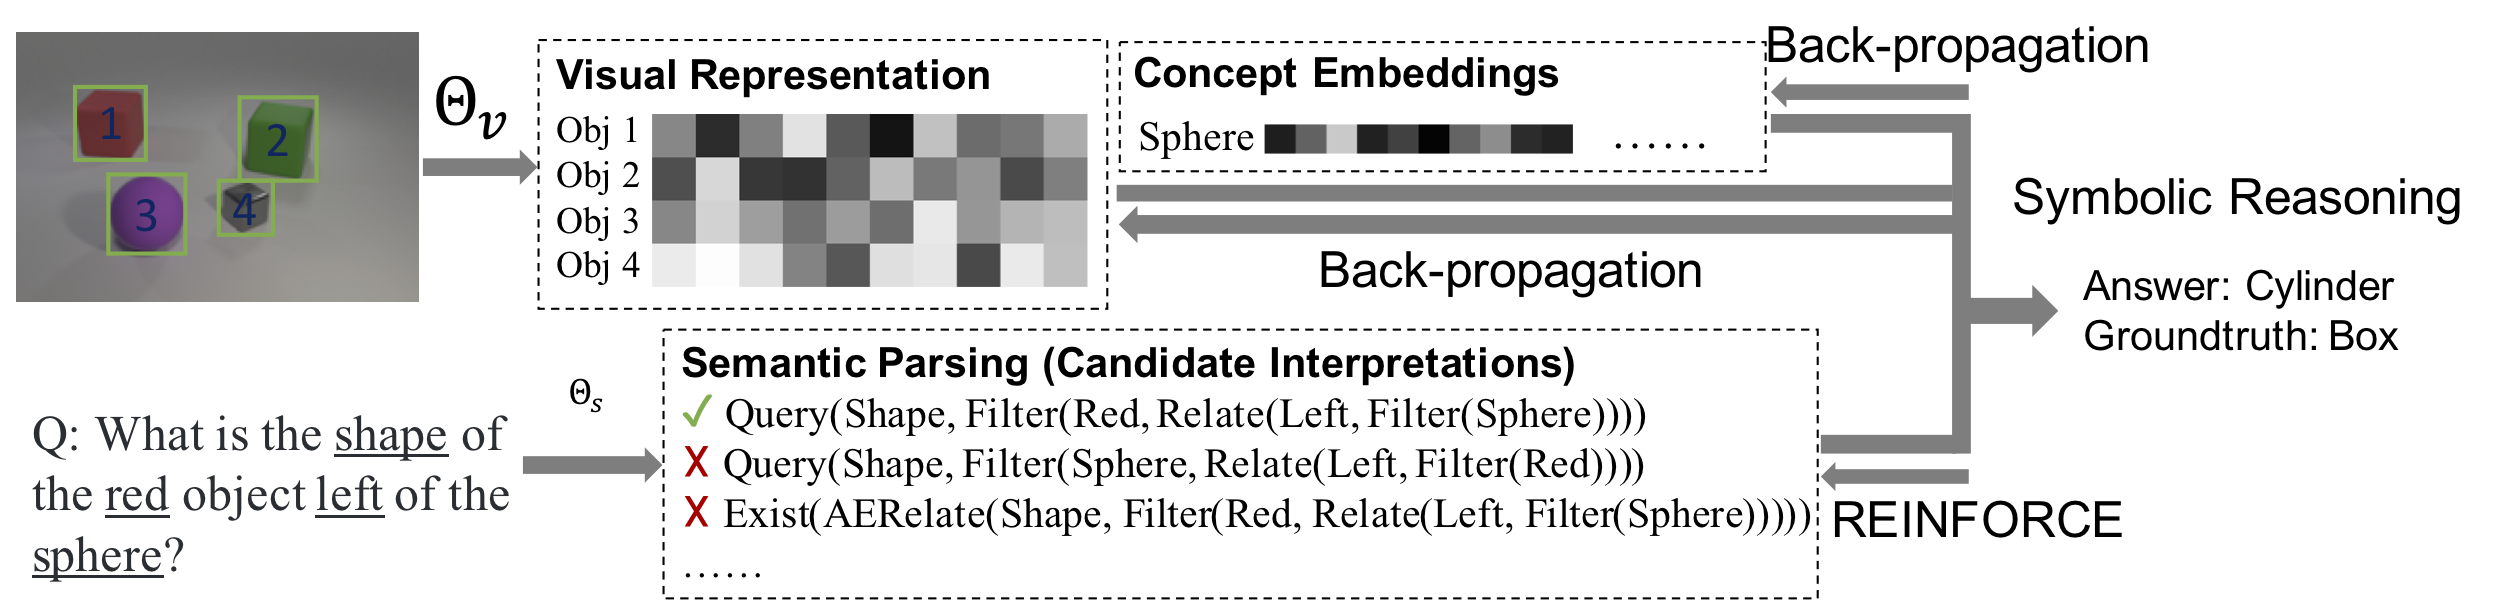
\includegraphics[width=\textwidth]{assets/nscl.png}
    \caption{Neuro-symbolic Concept Learner}
    \label{fig:nscl}
\end{figure}

\subsubsection{Semantic image manipulation from scene graphs \cite{dhamo2020_SIMSG}}

SIMSG provides a framework for image manipulation using scene graphs. The approach consists of the following steps, as can be seen in figure \ref{fig:simsg}
\begin{itemize}
    \item Modifying the scene graph of the image and passing it to a spatio-semantic scene graph network
    \item Constructing a 2D spatial arrangement of features, called the scene layout, by placing features of each object at their location in the image, determined by the predicted bounding boxes and masks
    \item Synthesise the final image from the scene layout via a neural decoder, conditioned on the initial image. 
\end{itemize}
The training is done by masking parts of the original image, and then tasking the model to reconstruct the whole image, thus removing the need for a dataset with explicit image manipulations.

\begin{figure}
    \centering
    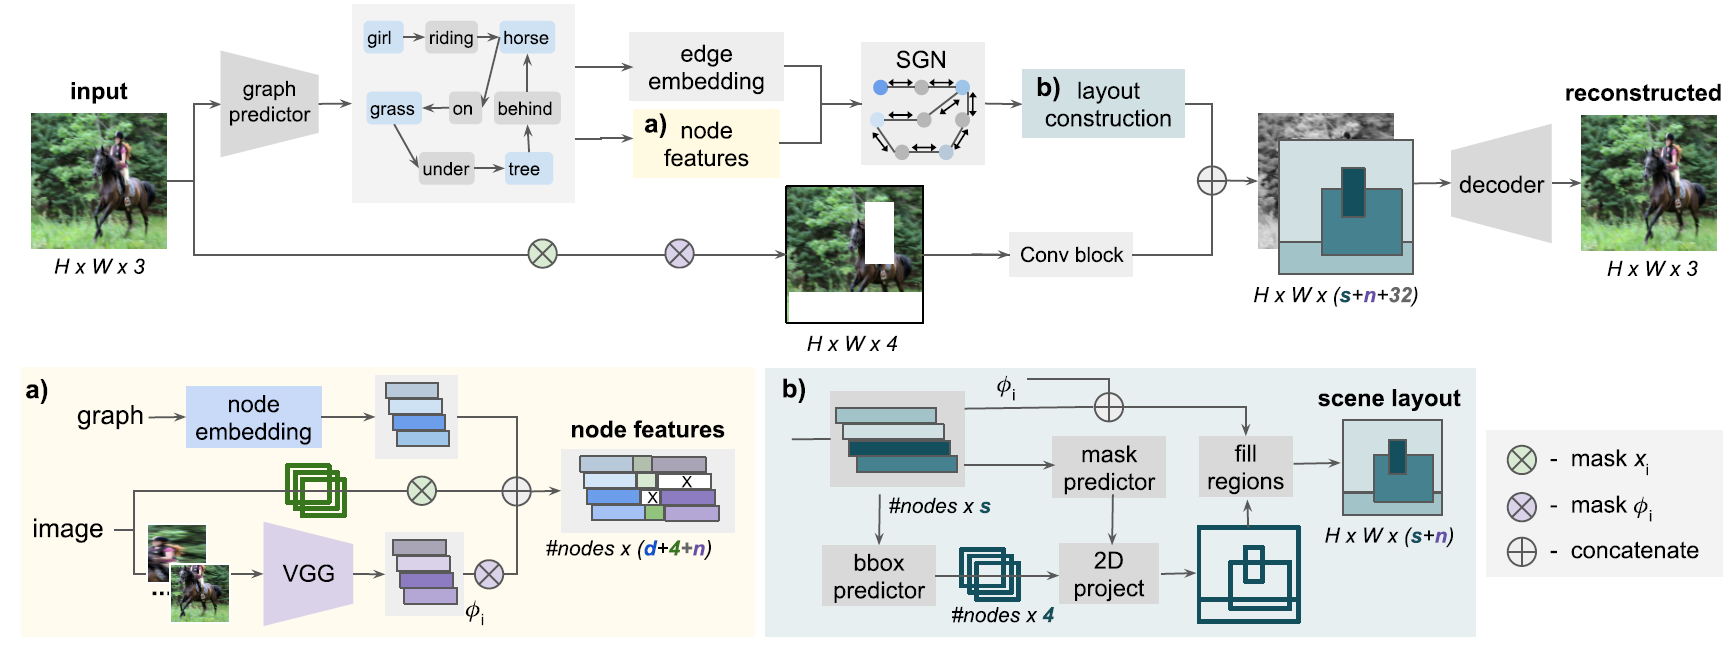
\includegraphics[width=\textwidth]{assets/simsg.png}
    \caption{Semantic Image Manipulation from Scene Graphs}
    \label{fig:simsg}
\end{figure}
